Los resultados principales se resumen en las figuras estaticas globales y en los grafos `joint_no_density` y `joint` con lens pca2. La configuracion con mayor complejidad combinada fue `orbital_pca2_cubes10_overlap0p35`, con 124 nodos y beta_1=96. Esto no prueba clases planetarias finales: resume estructura inducida por una matriz completada y auditada. \begin{figure}[H]\centering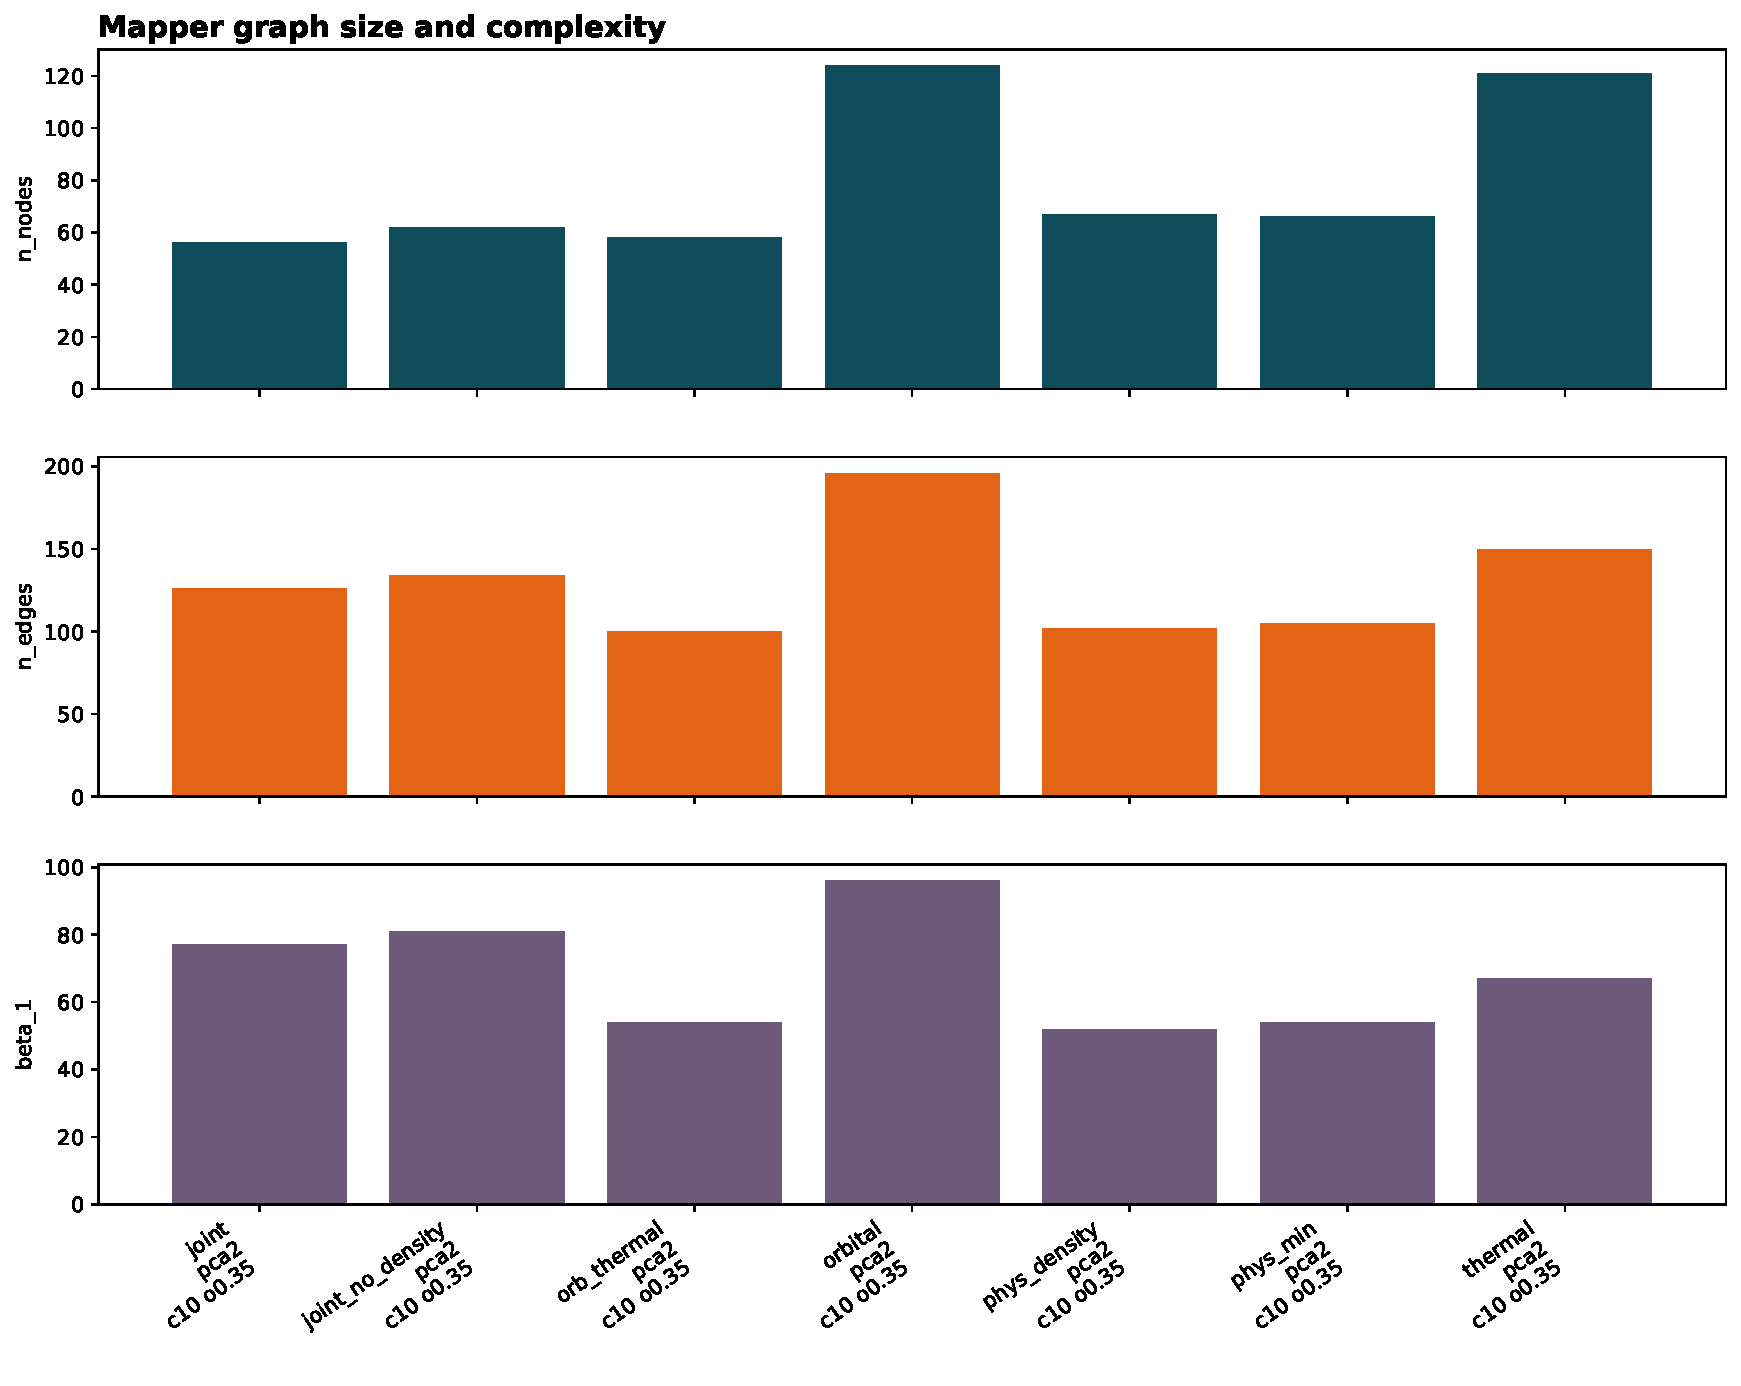
\includegraphics[width=0.95\linewidth]{figures/01_mapper_graph_size_complexity.pdf}\caption{Tamano y complejidad de los grafos Mapper.}\end{figure}\begin{figure}[H]\centering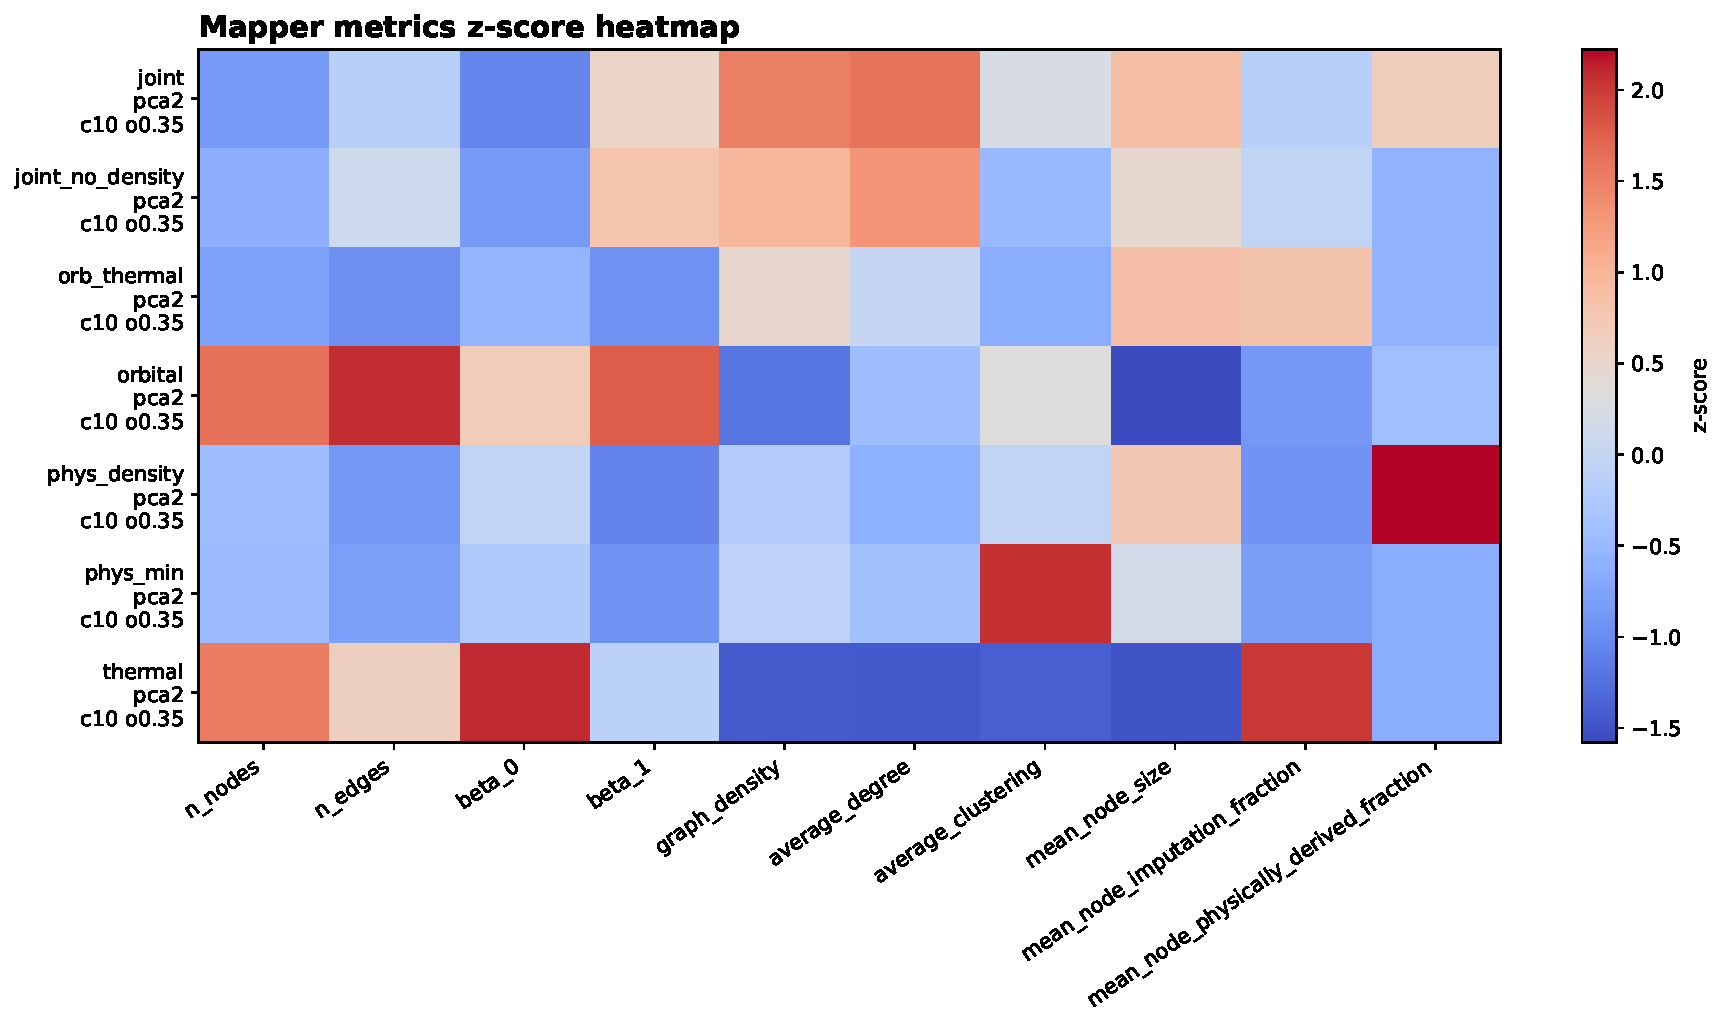
\includegraphics[width=0.95\linewidth]{figures/02_mapper_metrics_zscore_heatmap.pdf}\caption{Heatmap de metricas estandarizadas.}\end{figure}\begin{figure}[H]\centering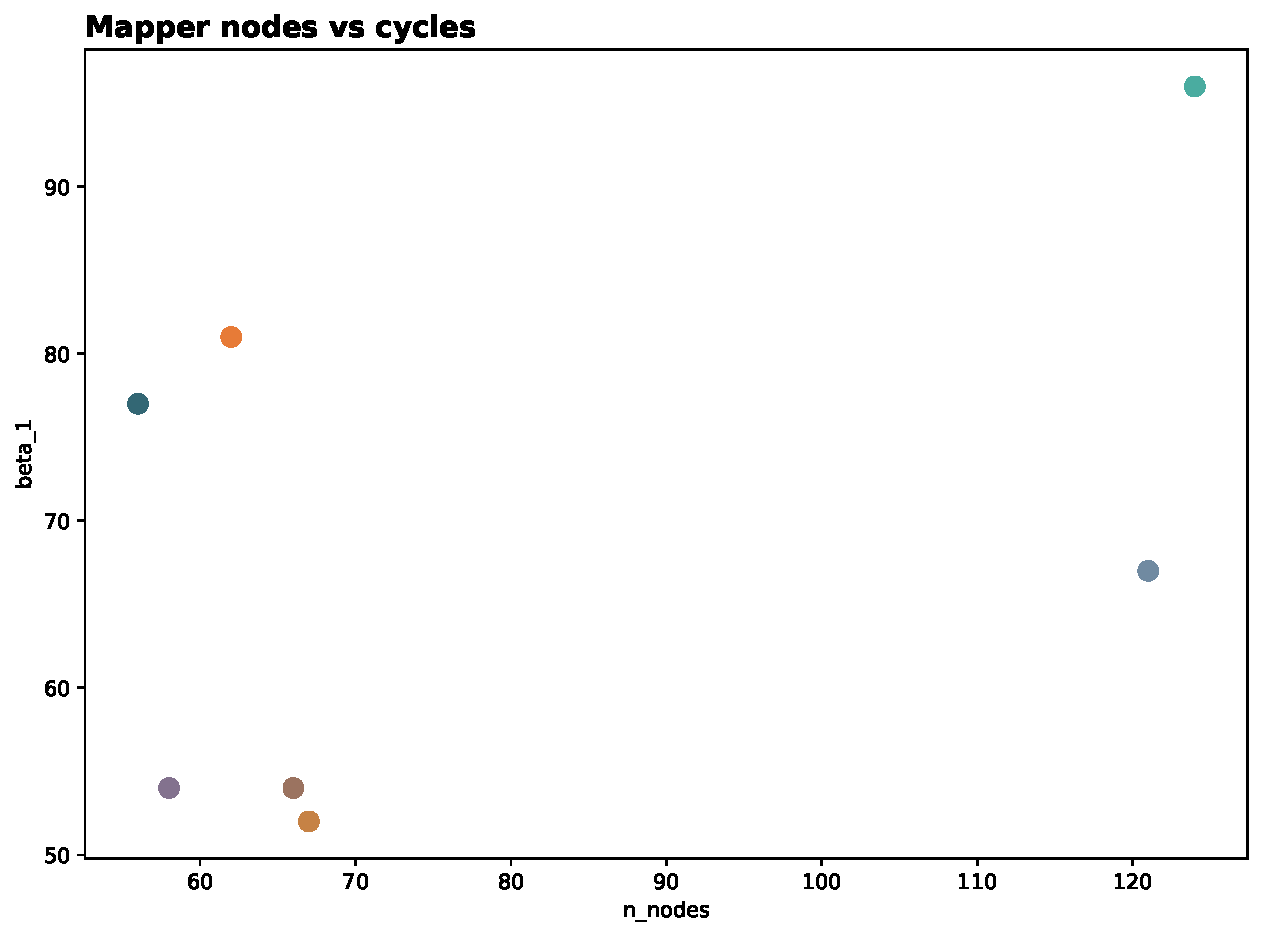
\includegraphics[width=0.75\linewidth]{figures/04_mapper_nodes_vs_cycles.pdf}\caption{Relacion entre numero de nodos y ciclos.}\end{figure}
